% -*- root: ../mnedo.tex -*-
\section{Hoja 1}
\begin{problem}[1]
Considerar el PVI:
\[\left\{ \begin{array}{l}y'=f(t) \ t \in [t_0,T] \\
y(t_0)=0\end{array}
\right.\]

Probar que utilizando el método de Euler:
\[y_N=\sum_{k=0}^{N-1} f(t_k)h\]
\solution

Recordamos que el método de Euler consiste en emplear
\[y_{n+1} = y_n + h f(t_n)\]

Por inducción podemos resolverlo:

\begin{equation*}
	\begin{multlined}[0.8\textwidth]
		\underline{n=0}: \quad y_1=y_0+hf(t_0) = h(t_0)\\[1em]
		\shoveleft{\underline{n=1}: \quad y_2 = y_1 + hf(t_1) = hf(t_0) + hf(t_1)}\\
		\shoveleft{\qquad \qquad \quad = h\left[ f(t_0) + f(t_1) \right]}\\
	\end{multlined}
\end{equation*}

La hipótesis de inducción es que: $y_N = \sum_{k=0}^{N-1} f(t_k)h$. Así que solo nos falta demostrar que se cumple en $N+1$:
\[y_{N+1} = y_N + hf(t_N) = \sum_{k=0}^{N-1} f(t_k)h + hf(t_N) = \sum_{k=0}^N f(t_k)h\]

\end{problem}


\begin{problem}[2]
Ver que el método de Euler falla cuando queremos aproximar la solución
\[y(t) = t^{\frac{3}{2}}\]
del PVI
\[\left\{ \begin{array}{l}y'=\frac{3}{2}y^{\frac{1}{3}} \\
y(0)=0\end{array}
\right.\]

Justifica cuál es el problema.

\solution
\doneby{Pedro}

Recordamos que el método de Euler consiste en emplear
\[y_{n+1} = y_n + h f(y_n)\]

Puesto que el dato inicial es 0 y no hay ninguna constante positiva sumando en la $f(t_n,y_n)$, todas las $y_n$ que calculemos tendrán valor 0 con lo que el método no nos llevará a ningún sitio.

Si el método de Euler no nos lleva a ningún sitio, parece lógico pensar que la función debe tener algún problema que la hace salir del conjunto de funciones sobre las que se puede emplear este método.

Así parece lógico pensar que la función $f(t_n,y_n)=\frac{3}{2}y^{\frac{1}{3}}$ no es lipschitz en la segunda variable. Vamos a comprobarlo.

Sea $L$ la constante que define la condición de Lipchitz, siendo el intervalo en el que estamos trabajando el intervalo $[0, \infty)$.

Tomamos en concreto $y_1=0$. En estas condiciones, si la función fuese Lipchitz tendríamos que
\[\frac{\frac{3}{2}(y_2^{1/3})}{y_2} = \frac{3}{2}\frac{1}{y^{2/3}}\leq L y_2 \ \ \ \forall y_2 \in [0,\infty)\]

Llegados a este punto es sencillo ver que la parte de la izquierda tiende a infinito cuando $y_2$ tienda a 0 y por tanto no puede existir la constante $L$ que lo acote. Por tanto la función no es Lipchitz y no podemos aplicar el método de Euler.
\end{problem}

\begin{problem}[3]
Sea el PVI
\[\left\{ \begin{array}{l}y'=1+y^2 \ t \in [0,2] \\
y(0)=0\end{array}
\right.\]

¿Podemos usar el método de Euler para aproximar la solución $y(t)=\tan(t)$?

\solution

Para empezar debemos de comprobar si la función que queremos aproximar satisface la ecuación planteada en el PVI.

\[\tan(x)' = \sec(x)^2 = 1 + \tan(x)^2, \ \ \tan(0)=0\]

Queda claro que el PVI planteado tiene como solución la función tangente. Ahora tenemos que ver si el problema planteado puede resolverse por el método de Euler.

Para verlo debemos comprobar si la función $f(t_n,y_n)=1+y^2$ es lipschitz en la segunda variable. Sólo en caso de serlo podríamos aplicar el método de Euler para obtener la solución. Vamos a ello.

\[\forall y_1<y_2 \in [0,2] \ \ \frac{\abs{y_2^2 - y_1^2}}{y_2-y_1}=\frac{(y_2-y_1)(y_2+y_1)}{y_2-y_1} = (y_2+y_1)< \infty\]

\obs No podemos acotar la suma $y_1+y_2$ porque no sabemos en que rango se mueve la $y$, puesto que sólo tenemos un dominio de definición para las $t$. Además, conisderando que conocemos la solución del método podemos comprobar que $\tan\left(\frac{π}{2}\right)=\infty$ con lo que la función claramente no es Lipschitz.

Por tanto, no podremos aproximar la función $y(t)=\tan(t)$ en ningún intervalo que contenga múltiplos enteros de $t=\frac{π}{2}$ puesto que en esos valores la función toma un valor infinito que nuestro método numérico no puede obtener.
\end{problem}


\begin{problem}[4]
Calcular el residuo de los siguientes métodos:

\ppart Regla del trapecio:
\[y_{n+1} = y_n + \frac{h}{2}\left( f(t_{n+1},y_{n+1})+f(t_n,y_n)\right)\]

\ppart Euler modificado:
\[y_{n+1} = y_n +hf\left( t_n+\frac{h}{2}, y_n+\frac{h}{2}f(t_n,y_n)\right)\]

\ppart Leap-frog
\[y_{n+2}=y_n+2hf(t_{n+1},y_{n+1})\]
\solution

\doneby{Pedro}

El residuo no es más que la diferencia entre el valor real de la función en $x_n$ y su valor aproximado a partir del método, es decir:
\[R_n = y(x_{n+1})-y_{n+1}\]

\spart
\[R_n = y(x_{n+1})-y_{n+1} = y(x_{n+1})-y(x_n) - \frac{h}{2}\left( y'(x_{n+1})+y'(x_n)\right)\]

Por Taylor podemos ver que:
\[\left\{\begin{array}{l}
y(x_{n+1}) = y(x_n)+hy'(x_n)+\frac{h^2}{2}y''(x_n)+O(h^3) \\
y'(x_{n+1}) = y'(x_n)+hy''(x_n) +O(h^2)
\end{array}\right.\]

Sustituyendo estos datos en la fórmula del residuo llegamos a:
\[R_n = O(h^3)\]

Puesto que el orden del método viene dado por $\frac{R_n}{h}$, en esta ocasión tenemos que el método del trapecio tiene un orden de consistencia al menos $2$.

Si realizásemos los desarrollos de Taylor con un orden mayor veríamos que el residuo deja de poder expresarse como $O(h^i)$, es decir, deja de estar controlado por $h$ con lo que podemos confirmar que el orden de consistencia del método es 2.

\spart

En esta ocasión
\[R_n = y(x_{n+1})-y(x_n)-hf\left( t_n+\frac{h}{2}, y_n+\frac{h}{2}y'(x_n)\right)\]

Calculando el desarrollo de Taylor de la $f$ llegamos a:
\[f\left( t_n+\frac{h}{2}, y_n+\frac{h}{2}y'(x_n)\right) = f(x_n,y_n)+\frac{h}{2}f_x(x_n,y_n)+\frac{h}{2}y'(x_n)f_y(x_n,y_n)= \atop y'(x_n)+\frac{h}{2}y''(x_n)+O(h^2)\]

Sustituyendo en la fórmula del residuo llegamos a:
\[R_n = O(h^3)\]

Si encomendamos nuestro alma al diablo y tratamos de estudiar si el residuo es de orden 3 vemos que no lo es, con lo que queda claro que el residuo es de orden 3 y por tanto el método es consistente de orden 2.

\spart

En esta ocasión
\[R_n = y(x_{n+2})-y(x_n)-2hy'(x_{n+1})\]

Desarrollando por Taylor el primer sumando tenemos
\[\left\{ \begin{array}{l}
y(x_{n+2}) = y(x_n) + 2hy'(x_n)+2h^2y''(x_n)+O(h^3) \\
y'(x_{n+1}) = y'(x_n)+hy''(x_n) + O(h^2)
\end{array}\right.\]

Y sustituyendo en la fórmula del residuo llegamos a:
\[R_n=O(h^3)\]


\end{problem}

\begin{problem}[5]
Dado $α \in [0,1]$ encontrar el orden del método:
\[y_{n+1} = y_n +hf(t_n+(1-α)h, αy_n+(1-α)y_{n+1})\]

\solution

Lo que debemos hacer es calcular el residuo cuya definición, recordemos, era:

\begin{defn}[Residuo]
Cuánto de lejos está la solución de satisfacer en un paso la fórmula de recurrencia
\end{defn}

Según esta definición, nuestro residuo será:
\[R_n = \underbrace{y(t_{t+1})}_{\label{ej1-5_tresTerminos}1} - \left\{ \underbrace{y(t_n)}_{2} + \underbrace{hf(t_n+(1-α)h, αy(t_n)+(1-α)y(t_{n+1}))}_{3} \right\}\]

Para conocer el orden de este residuo nos serviremos de los desarrollos de Taylor:
\[\hyperref[ej1-5_tresTerminos]{1} \quad y(t_{n+1}) = y(t_n)+y'(t_n)h + y''(t_n)\frac{h^2}{2} + O(h^3)\]

La segunda variable para la $f$ que aparece en \hyperref[ej1-5_tresTerminos]{3} se puede desarrollar como:
\[αy(t_n) + (1-α)y(t_{n+1}) = αy(t_n) + (1-α)\left[y(t_n) + y'(t_n)h +  y''(t_n)\frac{h^2}{2} + O(h^3) \right] \]
\[\qquad \qquad \qquad \qquad = y(t_n) + (1-α)\left[ y'(t_n)h + y''(t_n) \frac{h^2}{2} + O(h^3) \right]\]

Por tanto el desarrollo de Taylor de \hyperref[ej1-5_tresTerminos]{3} puede expresarse de la siguiente forma:

\[h\left( f(t_n,y(t_n))+\underbrace{f_x(t_n,y(t_n))\cdot (1-α)h +\underbrace{f_y(t_n,y(t_n))(1-α)h\left( y'(t_n)+y''(t_n)\frac{h}{2}+O(h^3)\right)}_{f_y(t_n,y(t_n))y'(t_n)(1-α)h + O(h^2)}}_{(1-α)h y''(t_n) + O(h^2)}\right) = \]

\[=hy'(t_n)+(1-α)h^2y''(t_n)+O(h^3)\]

De modo que las 3 expresiones las tenemos como:
\begin{equation*}
	\begin{multlined}[.8\textwidth]
		\hyperref[ej1-5_tresTerminos]{1} =  \quad y(t_{n+1}) = y(t_n) + y'(t_n) h + y''(t_n) \frac{h^2}{2} + O(h^3) \\
		\shoveleft{\hyperref[ej1-5_tresTerminos]{2} =  \quad y(t_n)} \\
		\shoveleft{\hyperref[ej1-5_tresTerminos]{2} =  \quad hy'(t_n) + (1-α) h^2 y''(t_n) + O(h^3)}\\
	\end{multlined}
\end{equation*}


Sumando \hyperref[ej1-5_tresTerminos]{1} y \hyperref[ej1-5_tresTerminos]{3}, y restando \hyperref[ej1-5_tresTerminos]{2} obtenemos:
\[R_n = y''(t_n)h^2 \left(\frac{1}{2}-(1-α) \right)+O(h^3)\]


Ahora tenemos dos casos posibles, y sabiendo que el orden de un método es $\frac{R_n}{h}$:
\begin{itemize}
\item α=1/2
\[R_n=O(h^3) \implies \text{ orden } \geq 2\]
\item α$\neq$1/2
\[R_n = y''(t_n)h^2 \left(\frac{1}{2}-(1-α) \right) + O(h^3) \implies \text{ orden } 1\]
\end{itemize}

\end{problem}


\begin{problem}[6]
	\ppart Sea un PVI. Utilizando los polinomios de interpolación de Lagrange obtener el método de Adams-Bashforth de dos pasos
	\[y_{n+2} = y_{n+1} + h \left( \frac{3}{2}f(t_{n+1}, y_{n+1}) + \frac{1}{2}f(t_n,y_n) \right),\]

	\ppart y el de tres pasos
	\[y_{n+3} = y_{n+2} + h \left( \frac{23}{12} f(t_{n+2},y_{n+2}) - \frac{4}{3} f(t_{n+1}, y_{n+1}) + \frac{5}{12}f(t_n,y_n) \right)\]

	\solution
	\begin{defn}{\textbf{Polinomio de interpolación de Lagrange}}

		Recordemos (de cálculo numérico) que el polinomio de interpolación de Lagrange tenía la forma:
		\[P(x) = f(x_0)l_0(x) + f(x_1)l_1(x) + … + f(x_N)l_N(x)\]
		donde $f$ es la función que queremos aproximar en los $x_i,\ i=0,…,N$ puntos, y
		\[l_i(x) = \frac{(x-x_0) … (x-x_{i-1}) (x-x_{i+1}) … (x-x_N)}{(x_i-x_0) … (x_i-x_{i-1}) (x_i-x_{i+1}) … (x_i-x_N)}\]
	\end{defn}

	\spart
	En el método de Adams Bashforth tenemos que
	\[y(x_{n+2})-y(x_{n+1}) = \int_{x_{n+1}}^{x_{n+2}} f(x,y(x)) dx\]
	y el valor de $f$ entre los puntos $x_{n+1}, x_{n+2}$ se aproximama mediante la recta que pasa por los puntos $((x_{n+1},f(x_{n+1},y_{n+1})), (x_{n+2}, f(x_{n+2},y_{n+2})))$. Para obtener dicha recta usamos el polinomio de interpolação de Lagrange:
	\[f(x,y) = f(x_n,y_n)\frac{x-x_{n+1}}{x_n-x_{n+1}} + f(x_{n+1},y_{n+1}) \frac{x-x_n}{x_{n+1}-x_n}\]

	Si integramos entre $\int_{x_{n+1}}^{x_{n+2}}$
	\[\int_{x_{n+1}}^{x_{n+2}} \left[ f(x_n,y_n)\frac{x_{n+1}-x}{h} + f(x_{n+1},y_{n+1})\frac{x-x_n}{h} \right]dx =\]
	\[= \left[ f(x_{n+1},y_{n+1}) \frac{(x-x_n)^2}{2h} - f(x_n,y_n)\frac{(x_{n+1}-x)^2}{2h} \right]_{x_{n+1}}^{x_{n+2}}  =\]
	\[= \frac{1}{2h}f(x_{n+1},y_{n+1}) \left[ (x_{n+2}-x_n)^2 - (x_{n+1}-x_n)^2 \right] - \frac{1}{2h} \left[ (x_{n+1} - x_{n+2})^2 - (x_{n+1} - x_{n+1})^2 \right] =\]
	\[= \frac{h}{2} \left( 3f(x_{n+1},y_{n+1}) - f(x_n,y_n) \right)\]


	\spart
	En este caso tendremos que:
	\[y_{n+1} - y_n = \int_{x_n}^{x_{n+1}} f(x,y(x)) dx\]
	Con la particularidad de que ahora la aproximación de $f$ en el intervalo $[x_n,x_{n+1}]$ la realizaremos interpolando la $f$ en los puntos $x_{n-2},x_{n-1},x_n$ con el polinomio de Lagrange $p$.

	Sabemos por tanto que $p$ interpola $f$ en $x_{n-2},x_{n-1},x_n$:

	\begin{center}
	\inputtikz{EJRC_interpolar}
	\end{center}

	Para simplificar los cálculos vamos a tomar el cambio de variable $u=\frac{x_{n+1}-x}{h}$ para que así el polinomio interpole $f(u,y(u))$ en los puntos $3,2,1$. ($u(x_{n-2})=3, u(x_{n-1})=2, u(x_n)=1$).

	\begin{center}
	\inputtikz{EJRC_interpolar_transformed}
	\end{center}


	Es decir, tras el cambio de variable el polinomio interpolador queda como

	\[\tilde{p}(u) = f(x_n,y_n) \frac{(u-2)(u-3)}{(1-2)(1-3)} + f(x_{n-1},y_{n-1}) \frac{(u-1)(u-3)}{(2-1)(2-3)}+f(x_{n-2},y_{n-2}) \frac{(u-1)(u-2)}{(3-1)(3-2)}\]

	De modo que tras el cambio de variable tendremos:
	\[\int_{x_n}^{x_{n+1}}p(x)dx \underbrace{=}_{t_{n+1}-hu=x} h\int_0^1 p(t_{n+1}-hu) du = h\int_0^1 \tilde{p}(u)du =\]
	\[= h\int_0^1 \left[ f(x_n,y_n) \frac{(u-2)(u-3)}{(1-2)(1-3)} + f(x_{n-1},y_{n-1}) \frac{(u-1)(u-3)}{(2-1)(2-3)}+f(x_{n-2},y_{n-2}) \frac{(u-1)(u-2)}{(3-1)(3-2)} \right] =\]
	\[= h\int_0^1 \left[ f(x_n,y_n)\frac{u^2-5u+6}{2} - f(x_{n-1},y_{n-1})(u^2-4u+3) + f(x_{n-2},y_{n-2})\frac{u^2-3u+2}{2} \right] =\]
	\[=  h \left( \frac{23}{12} f(t_{n+2},y_{n+2}) - \frac{4}{3} f(t_{n+1}, y_{n+1}) + \frac{5}{12}f(t_n,y_n) \right)\]

	Por tanto
	\[y(x_{n+2})-y(x_{n+1}) = \int_{x_{n+1}}^{x_{n+2}} p(x) dx = h \left( \frac{23}{12} f(t_{n+2},y_{n+2}) - \frac{4}{3} f(t_{n+1}, y_{n+1}) + \frac{5}{12}f(t_n,y_n) \right)\]
\end{problem}

\begin{problem}[7]
La regla de integración del trapecio se define por:

\[y_{n+1} = y_n + \frac{h}{2}\left( f(t_{n+1},y_{n+1})+f(t_n,y_n)\right)\]

Probar que la regla del trapecio es 0-estable. Nótese que basta con demostrar que la función incremento asociada a esta regla, $\phi(t,y;h)$ cumple:
\begin{enumerate}
\item Es continua con respecto a las variables $t,y,h$
\item Es Lipschitz con respecto a la variable $y$
\item Si $f=0$, entonces $\phi_f=0$
\end{enumerate}
\solution

\doneby{Pedro}

Técnicamente el ejercicio está hecho en clase pero yo me preocupé de copiarlo aquí de nuevo.

\begin{itemize}
\item Es continua con respecto a las variables $t,y,h$

Definimos la aplicación global contractiva
\[F(\phi) = \frac{1}{2} \left[ f(x_n,y_n) + f(x_{n+1}, y_n+h\phi) \right]\]

Y tomamos $\phi_f = \lim_{j\to∞} \phi_f^{[j]}$, donde $\phi_f^{[j]}$ viene dada por la sucesión $\phi_f^{[j]} = F\left(\phi_f^{[j-1]}\right)$ y $\phi^0 = 0$.

\obs El método del trapecio es de 1 paso ($k=1$) y por tanto la función incremento solo depende de $x_n$, $y_n$ y $h$, es decir $\phi_f(x_n,y_n;h)$.

Dado que $f$ es una función continua, tendremos que la función:
\[\phi_f^{[1]}(x_n,y_n;h) = \frac{1}{2} \left[ f(x_n,y_n) + f(x_{n+1}, y_{n+1} + 0) \right]\]
será continua. Como la composición de funciones continuas da como resultado otra función continua, tendremos que $\phi_f^{[2]}=F\left( \phi_f^{[1]} \right)$ es continua, y por tanto todas las $\phi_f^{[k]}(x_n,y_n;h)$ son continuas.

Si logramos probar que la convergencia de las $\phi_f^{[j]}$ sea uniforme, tendremos que la sucesión convergería a una función $\phi_f$ continua.

Expresamos $\phi_f^{[k]}$ como una suma telescópica:
\begin{equation}
	\label{eq:suma_telesc_pto_fijo_ej}
	\phi_f^{[k]} = \sum_{j=1}^k \phi_f^{[j]} - \phi_f^{[j-1]} + \phi_f^{[0]},\quad \phi_f^{[0]}=0
\end{equation}
Tomando la norma $L^∞$:
\begin{equation*}
	\begin{multlined}[0.7\textwidth]
		\md{\phi_f^{[j]} - \phi_f^{[j-1]} }_{L^∞} = \md{F\left[\phi_f^{[j-1]}\right] - F\left[\phi_f^{[j-2]}\right] }_{L^∞}\\[1em]
		\shoveleft{\qquad \qquad \qquad \underbrace{≤}_{F\text{ contractiva}} \frac{Lh}{2} \md{\phi_f^{[j-1]} - \phi_f^{[j-2]}}_{L^∞}}\\
	\end{multlined}
\end{equation*}
Aplicando la desigualdad sucesivamente:
\[\md{\phi_f^{[j]} - \phi_f^{[j-1]}}_{L^∞} ≤ \left(\frac{Lh}{2}\right)^{j-1} \md{\phi^{[1]}}_{L^∞}\]

Puesto que $K = [a,b]×ℝ×(0,∞)$ es compacto:
\[\md{\phi_f^{[j]} - \phi_f^{[j-1]}}_{L^∞} ≤ M_k\left(\frac{Lh}{2}\right)^{j-1}\]

De modo que aplicando el test $M$ de Weierstrass, la convergencia de \ref{eq:suma_telesc_pto_fijo_ej} es uniforme, y por tanto $\phi_f$ es continua.

\item Es Lipschitz con respecto a la variable $y$

%En el apartado anterior hemos visto que podemos construir una sucesión de funciones que converge uniformemente a $\phi_f$. Todas estas funciones seran funciones Lipschitz con respecto a la $y$ (que es la segunda variable de $\phi_f$) y por tanto todas las $\phi_f^{[j]}$ son Lipschitz.

%Puesto que la convergencia es uniforme, el límite también es una función Lipschitz.

%Vamos a demostrar esta afirmación para los lectores incrédulos.
%\begin{proof}
%De forma general vamos a considerar una sucesión de funciones $f_x(x,y)$ que converge uniformemente a $f(x,y)$.

%Por definición de convergencia uniforme, tenemos:
%\[\forall ε > 0 \exists n \tq \forall N > n \ \ \norm{f(x,y)-f_n(x,y)} \leq ε\]

%Vamos a estudiar ahora la ``Lipschitzialidad'' de la función $f$ sabiendo que todas las $f_n$ son Lipschitz.

%\[\norm{f(x,y)-f(x,y')} = \norm{f(x,y)\pm f_n(x,y)\pm f_n(x,y')+f(x,y')} \leq \]
%por la desigualdad triangular
%\[\leq \norm{f(x,y)-f_n(x,y)}+\norm{f(x,y')-f_n(x,y')}+\norm{f_n(x,y)-f_n(x,y')} = \atop 2ε +\norm{f_n(x,y)-f_n(x,y')}\]

%Finalmente, puesto que las $f_n$ son Lipschitz tenemos que:
%\[2ε +\norm{f_n(x,y)-f_n(x,y')} \leq 2ε + \norm{y-y'}\]

%Puesto que $\forall ε > 0$ podemos encontrar un $n$ que nos permita llevar a cabo estas operaciones, podemos hacer ε tan pequeño como queramos y llegar a:
%\[\norm{f(x,y)-f(x,y')} \leq \norm{y-y'}\]
%\end{proof}
Por definición, para el método del trapecio tenemos que $\phi_f$ es la solución de
\[\phi_f (x_n,y_n) = \frac{h}{2}\left(f(x_n,y_n)+f(x_{n+1},y_{n+1}) \right) = \frac{1}{2}\left( f(x_n,y_n) + f(x_{n+1},y_n+h\phi_f(x_n,y_n)\right)\]

Con la definición de $\phi_f$ podemos escribir
\[\norm{\phi_f(x_n,y_n,h)-\phi_f(x_n,\tilde{y}_n,h)}  \leq \]
\[\leq \frac{1}{2}\norm{f(x_n,y_n)-f(x_n,\tilde{y}_n)}+\frac{1}{2}\norm{f(x_{n+1},y_n+h\phi_f(x_n,y_n))-f(x_{n+1},\tilde{y}_n+h\phi_f(x_n,\tilde{y}_n))} \leq\footnote{por ser $f$ Lipschitz}\]
\[\leq L\norm{y_n-\tilde{y}_n}+\frac{Lh}{2}\norm{\phi_f(x_n,y_n,h)-\phi_f(x_n,\tilde{y}_n,h)}\]

Reordenando los términos de la inecuación podemos escribir:
\[\left(1-\frac{Lh}{2} \right)\norm{\phi_f(x_n,y_n,h)-\phi_f(x_n,\tilde{y}_n,h)} \leq L\norm{y_n-\tilde{y}_n}\]
\item Si $f=0$, entonces $\phi_f=0$

Puesto que en el método del trapecio $\phi_f$ se define como el punto fijo de
\[F(\phi) = \frac{1}{2} \left[ f(x_n,y_n) + f(x_{n+1}, y_n+h\phi) \right]\]

si $f=0$ tendremos que $\phi_f$ será el punto fijo de la función nula y, por tanto, será 0

\end{itemize}
\end{problem}

\begin{problem}[8]
Probar que los métodos de Adams-Bashforth de dos pasos y de tres pasos, definidos en el ejercicio 6, son convergentes.
\solution

\doneby{Jorge}

En este ejercicio primero probaremos que los métodos son consistentes usando el teorema \ref{theorem:consist_iif_relaciones}. Después probaremos que son 0-estables, y sirviéndonos del teorema \ref{theorem:consist_y_0estable_converge} podremos decir que el MN es convergente.

Este ejercicio lo hicimos antes de conocer el criterio de la raíz \ref{theorem:criterio_raiz}, que simplifica enormemente la demostración de la 0-estabilidad. Al final de cada apartado se encuentra la versión del profesor, que emplea este criterio.
\textcolor{red}{
\obs Para poder aplicar los teoremas vistos en clase sobre métodos numéricos, antes debemos comprobar que el método con el que trabajamos satisface las hipótesis de un buen método numérico y, por tanto, los teoremas son válidos.}

\spart \textbf{Método de 2 pasos}:

El método de Adams-Bashforth de dos pasos se trata de un método basado en cuadratura que emplea la relación
\[y(x_{n+2}) - y(x_{n+1}) = \int_{x_{n+1}}^{x_{n+2}} f(x,y(x)) \dif x\]

donde $f(x,y(x))$ se aproxima por medio de la recta interpolante entre los puntos $(x_n,y(x_n))$ y $(x_{n+1},y(x_{n+1}))$, es decir:
\[f(x,y(x)) \approx f(x_n, y(x_n)) \frac{x-x_{n+1}}{x_n-x_{n+1}}+f(x_{n+1},y(x_{n+1}))\frac{x-x_n}{x_{n+1}-x_n}\]

Finalmente, el método queda expresado como:
\[y_{n+2} = y_{n+1}+\frac{h}{2}\left( 3f(x_{n+1},y_{n+1})-f(x_n,y_n)\right)\]

\textbf{El ejercicio propiamente dicho empieza a partir de esta última igualdad, lo anterior sólo era para entrar en calor}

\begin{enumerate}
\item \textbf{Consistencia}

Es sencillo ver que \[\sum_{j=0}^{k=2} α_j = 0 - 1 + 1 = 0\]

Para este método, tenemos la función incremento
\[\phi_f(x_n,y_n,h) = \frac{1}{2}\left(3f(x_n+h,y_n+h\phi_f(x_n,y_n,h))-f(x_n,y_n)\right)\]

De donde podemos ver que:
\[\phi_f(x,y(x),0) = \frac{1}{2} \left(3f(x,y(x)) - f(x,y(x)) \right) = f(x,y(x))\]

Para poder aplicar el teorema \ref{theorem:consist_iif_relaciones} necesitamos ver que:
\[\phi_f(x,y(x),0)  = \sum_{j=0}^2jα_jf(x,y(x))=-f(x,y(x)) + 2 f(x,y(x)) = f(x,y(x))\]

Por tanto, podemos aplicar el teorema \ref{theorem:consist_iif_relaciones} y garantizar así que el método es consistente.

\item \textbf{0-estabilidad}

Consideramos dos sucesiones: $\left\{ y_n \right\}_{n=0}^N$, $\left\{ y(x_n) \right\}_{n=0}^N$ y buscamos las sucesiones $δ_n,γ_n$ asociadas, que serán aquellas que satisfagan las ecuaciones:

\[\sum_{j=0}^kα_jy_{n+j} = h\phi_f(x_n,y_n,...,y_{n+j},h)+hδ_n\]
\[\sum_{j=0}^kα_jy(x_{n+j}) = h\phi_f(x_n,y(x_n),...,y(x_{n+j}),h)+hγ_n\]

Para poder garantizar la 0-estabilidad, por definición, debemos probar que
\[\max_{k \leq n \leq N}\norm{y_n - y(x_n)} \leq C\left( \max_{0 \leq n \leq k-1}\norm{y(x_n) - y_n}+\max_{0 \leq n \leq N-k}\norm{δ_n - γ_n}\right)\]

Por la propia definición del método numérico tenemos que $δ_n=0$. Vamos a estudiar la diferencia entre las sucesiones:

\[y(x_{n+2})-y_{n+2} = y(x_{n+2}) - y_{n+1} - \frac{h}{2}\left( 3f(x_{n+1},y_{n+1}) - f(x_n,y_n)\right)\]

Desarrollando con Taylor en torno a $x_n$ tenemos:
\[y(x_{n+2}) = y(x_n)+2hf(x_n,y(x_n))+O(h^2)\]
\[y_{n+1} = y_n +hf(x_n,y_n)+O(h^2)\]
\[f(x_{n+1},y_{n+1}) = y'_{n+1} = f(x_n,y_n) + O(h)\]

Sustituyendo en la diferencia tenemos:
\[y(x_{n+2})-y_{n+2} = y(x_n)-y_n+ h(2f(x_n,y(x_n))-f(x_n,y_n)) - hf(x_n,y_n)+ O(h^2) =\]
\[=y(x_n)-y_n+2h(f(x_n,y(x_n))-f(x_n,y_n)) + \underbrace{O(h^2)}_{\text{residuo = }hδ_n}\]

Ahora procedemos a acotar la diferencia:
\[\underbrace{\norm{y(x_{n+2})-y_{n+2}}}_{\max_{k \leq n \leq N}\norm{y_n - y(x_n)}} \leq \norm{y(x_n)-y_n} + 2hL\norm{y_n-y(x_n)}+hδ_n \leq \underbrace{(Kh)}_C\left(\underbrace{\norm{y_n-y(x_n)}}_{\max_{0 \leq n \leq k-1}\norm{y(x_n) - y_n}}+δ_n\right)\]

Con lo que vemos que, efectivamente, se cumple la condición de 0-estabilidad

\textbf{Versión del profesor}

Para estudiar la 0-estabilidad aplicamos el criterio de la raíz.

En esta ocasión el primer polinomio característico es $P(x)=x^2-x$, cuyas raíces son 0 y 1 con lo que, efectivamente se satisface el criterio de la raíz pues una raíz tiene módulo menor que 1 y la que tiene módulo 1 es simple.

\end{enumerate}

\spart \textbf{Método de 3 pasos}:

\begin{enumerate}
\item \textbf{Consistencia}

Se cumple la primera afirmación de la parte derecha de \ref{theorem:consist_iif_relaciones}:
\[\sum_{j=0}^{k=3} α_j = 1 - 1 + 0 + 0 = 0\]

En este caso $\phi_f(x_n,y_n,y_{n+1},y_{n+2}, h) = \frac{23}{12}f(x_n+2h, y_{n+2}) - \frac{16}{12}f(x_n+h,y_{n+1}) + \frac{5}{12}f(x_n,y_n)$, y por tanto se cumple la segunda afirmación de la parte derecha de \ref{theorem:consist_iif_relaciones}:
\[\phi_f(x,y(x),y(x),y(x), 0) = \frac{23}{12}f(x+2h, y(x)) - \frac{16}{12}f(x,y(x)) + \frac{5}{12}f(x,y(x)) = \overbrace{1}^{\sum_{j=0}^{k=3} jα_j} f(x,y(x))\]

\item \textbf{0-estabilidad}
Por tanto \textbf{el MN es 0-estable} y por tanto es consistente. Así que solo nos queda ver que el MN es 0-estable:

Tomamos las sucesiones $\left\{ y_n \right\}_{n=0}^N$, $\left\{ y(x_n) \right\}_{n=0}^N$ y las restamos:

\small
\begin{equation*}
	\begin{multlined}[\textwidth]
		y(x_{n+3}) - y_{n+3} = y(x_{n+2}) - y_{n+2} + h\frac{23}{12}\left(f(x_{n+2},y(x_{n+2})) - f(x_{n+2},y_{n+2})\right) + \\[1em]
		~
		\shoveleft{\qquad + h \left\{- \frac{16}{12}\left(f(x_{n+1},y(x_{n+1})) - f(x_{n+1},y_{n+1})\right) + h \frac{5}{12}\left(f(x_n,y(x_n)) - f(x_n,y_n)\right) \right\} + \overbrace{hδ_n}^{R_n}}\\
	\end{multlined}
\end{equation*}
\normalsize

Tomando valores absolutos a ambos lados y usando que $f$ es Lipschitz en la segunda variable:
\small
\begin{equation*}
	\begin{multlined}[\textwidth]
		\abs{y(x_{n+3}) - y_{n+3}} ≤ \\[1em]
		~
		\shoveleft{\qquad ≤ \abs{y(x_{n+2}) - y_{n+2}} + \frac{23}{12}Lh \left\{\abs{y(x_{n+2})-y_{n+2}} + \abs{y(x_{n+1})-y_{n+1}} + \abs{y(x_n)-y_n} \right\} + h\abs{δ_n} ≤}\\
		~
		\shoveleft{\qquad ≤ \left(1+\frac{23}{12}Lh\right) \left\{\abs{y(x_{n+2})-y_{n+2}} + \abs{y(x_{n+1})-y_{n+1}} + \abs{y(x_n)-y_n} + \abs{δ_n} \right\} ≤}\\
		\shoveleft{\qquad ≤ 3\left(1+\frac{23}{12}Lh\right) \left\{\max_{0≤j≤2}\abs{y(x_{n+j})-y_{n+j}} + \abs{δ_n} \right\}}\\
	\end{multlined}
\end{equation*}
\normalsize

Con lo que queda claro que el método es 0-estable

\textbf{Versión del profesor}

El primer polinomio característico es $P(x) = x^3-x^2$ que tiene como solución doble al 0 y como solución simple al 1, por lo que satisface el criterio de la raíz, lo que nos garantiza que el método es 0-estable.
\end{enumerate}

\end{problem}

\section{Problemas previos al primer parcial}

En esta sección incluimos todos los problemas realizados en clase a modo de preparación para el primer parcial, que no están incluidos en las hojas de ejercicios.

\begin{problem}[1]
Probar la convergencia del método de Euler sabiendo que es consistente:

\solution

Recordemos que el método de Euler es un método numérico que permite resolver un problemas de valor inicial mediante la recursión:
\[y_{n+1} = y_n + hf(x_,y_n)\]

Sabiendo esto, podemos ver que el residuo puede escribirse como:
\[y(x_{n+1}) = y(x_n) + hf(x_n,y_n) + R_n\]
que no es más que aplicar la definición de residuo.

Dado el dato inicial $y(0)=y^0$, para poder ver que el método es convergente debemos comprobar que:
\[\lim_{h \to 0 } \norm{y^0-y_0} \to 0 \implies \lim_{h\to 0} \max_{1 \leq n \leq N}\norm{y(x_n)-y_n} \to 0\]

\obs A lo largo de la teoría hemos realizado esta misma demostración asumiendo que $\norm{y^0-y_0} = 0$, pero esta restricción es demasiado fuerte puesto que en la práctica puede incluso llegar a ser imposible.

Basándonos en la fórmula recursiva del método podemos ver que:
\[y(x_{n+1}) - y_{n+1} = y(x_n) - y_n + hf(x_n,y(x_n)) -hf(x_n,y_n) + R_n\]
puesto que la función $f$ es Lipschitz, tomando módulos a ambos lados tenemos:
\[|y(x_{n+1})-y_{n+1}| \leq (1+Lh)|y(x_n)-y_n| + K \text{ siendo }K=\max_n|R_n|\]
Recordando la demostración que realizamos en teoría al probar el teorema \ref{theorem:EulerEsConvergente}
\[\max_n|y(x_n)-y_n| \leq C(L)|y^0-y_0|+C\frac{K}{h}\]

Así tenemos que
\[\lim_{h\to 0} \max_{1 \leq n \leq N}\norm{y(x_n)-y_n} \leq \lim_{h \to 0}\left( C(L)|y^0-y_0|+C\frac{K}{h}\right) \to 0\]
\end{problem}

\begin{problem}[2]
Demostrar, a lo bruto, que el método del trapecio es convergente

\solution

Sabemos que el método del trapecio viene definido por la recurrencia:
\[y_{n+1} = y_n +\frac{h}{2}\left(f(x_n,y_n)+f(x_{n+1},y_{n+1}) \right)\]

Para probar que el método es convergente necesitamos ver que:
\[\lim_{h \to 0 } \norm{y^0-y_0} \to 0 \implies \lim_{h\to 0} \max_{1 \leq n \leq N}\norm{y(x_n)-y_n} \to 0\]

Por definición del residuo podemos escribir:
\[y(x_{n+1}) - y(x_n) +\frac{h}{2}\left(f(x_n,y(x_n))+f(x_{n+1},y(x_{n+1})) \right) = R_n\]

Combinando esta ecuación con la recurrencia que define el método podemos escribir:
\[|y(x_{n+1})-y_{n+1}| \leq |y(x_n)-y_n|+\frac{h}{2}|f(x_n,y_n)-f(x_n,y(x_n))|+\frac{h}{2}|f(x_{n+1},y(x_{n+1}))-f(x_{n+1},y_{n+1})|+K\]

siendo $K=\max_{0 \leq n \leq k-1} R_n$

Puesto que sabemos que la función $f$ es Lipschitz podemos escribir:
\[|y(x_{n+1})-y_{n+1}| \leq \left( 1 + \frac{Lh}{2}\right)|y(x_n)-y_n|+\frac{Lh}{2}|y_{n+1}-y(x_{n+1})| + K\]
Agrupando los términos iguales a ambos lados de la desigualdad lleamos a:
\[\left(1- \frac{hL}{2}\right)|y(x_{n+1})-y_{n+1}| \leq \left(1+ \frac{hL}{2}\right)|y(x_n)-y_n| + K\]

Vamos ahora a tratar de encontrar la relación entre $|y(x_{n+1})-y_{n+1}|$ y $|y(x_0)-y_0|$ para lo que definimos $e_n=|y(x_{n})-y_{n}|$ lo que nos permite escribir:
\[e_{n+1} \leq \frac{\left(1+ \frac{hL}{2}\right)}{\left(1- \frac{hL}{2}\right)}e_n + \frac{1}{\left(1- \frac{hL}{2}\right)}K\]

Desarrollando la recurrencia podemos ver que:
\[e_{n+1} \leq \frac{\left(1+ \frac{hL}{2}\right)^n}{\left(1- \frac{hL}{2}\right)^n}e_0 + \frac{1}{\left(1- \frac{hL}{2}\right)}K\frac{\frac{\left(1+ \frac{hL}{2}\right)^n}{\left(1- \frac{hL}{2}\right)^n}-1}{\frac{\left(1+ \frac{hL}{2}\right)}{\left(1- \frac{hL}{2}\right)}-1}\]

\obs Para llegar a este resultado desarrollamos la recurrencia hasta ver su fórmula general. El coeficiente de $e_0$ es sencillo de obtener. Para el coeficiente de la $K$ necesitamos conocer la fórmula para la suma de los términos de una sucesión geométrica.

Por otro lado, podemos ver que:
\[\left( 1 + \frac{Lh}{2} \right)^n \leq \left( 1 + \frac{L(b-a)}{2N}\right)^N=\left(1 + \frac{L(b-a)}{2N}\right)^{\frac{2N}{L(b-a)}\frac{L(b-a)}{2}}\leq e^{\frac{L(b-a)}{2}}\]
\[\frac{1}{\left( 1-\frac{Lh}{2}\right)^n} \leq .. \leq e^{\frac{L(b-a)}{2}}\]
\[\frac{\left(1+ \frac{hL}{2}\right)}{\left(1- \frac{hL}{2}\right)}-1 = \frac{Lh}{1-\frac{Lh}{2}}\]

Combinando estos datos podemos escribir:
\[e_{n+1} \leq e^{L(b-a)}e_0+\frac{2K}{Lh}\left( e^{L(b-a)}-1\right) \leq C(L,b-a)\left( e_0 +\frac{K}{h}\right)\]

Así nos queda:
\[\max_{1\leq n \leq N} \norm{y(x_n)-y_n} \leq C(L,b-a)\left( \norm{y(x_0)-y_0} +\frac{K}{h}\right)\]

Y, por definición de la $K$ tenemos que:
\[K = \max_n |R_n|\]
Pero, sin realizar más asunción sobre la $f$ inicial más que su continuidad y conociendo la definición de residuo, tenemos que:
\[\lim_{h\to 0} \frac{K}{2} = \lim_{h \to 0} \frac{R_n}{h} = \lim_{h \to 0} y'(ε)-\frac{1}{2}y'(x_{n+1})-\frac{1}{2}y'(x_n) = 0 \text{ por continuidad de } y'=f\]

Finalmente podemos escribir:
\[\lim_{h\to 0}\max_{1\leq n \leq N} \norm{y(x_n)-y_n} \leq \lim_{h \to 0}C(L,b-a)\left( \norm{y(x_0)-y_0} +\lim_{h \to 0}\frac{K}{h}\right) \equiv\]
\[\equiv \lim_{h\to 0}\max_{1\leq n \leq N} \norm{y(x_n)-y_n} \leq \lim_{h \to 0}C(L,b-a) \norm{y(x_0)-y_0} \]

Con lo que queda claro que se satisface la condición de convergencia para este método de 1 paso
\end{problem}

\section{Hoja 2}
\begin{problem}[1]
Sea $A$ una matriz real cuadrada de orden $k$ definida de la siguiente manera:
\[\begin{array}{ll}
A(i,i+1) = 1 & \text{ para } i=1,...,k-1\\
A(k,j)=-\frac{α_{j-1}}{α_k} & \text{ para } j=1,...,k
\end{array}\]

Demostrar que su polinomio característico es:
\[ρ(λ) = \sum_{j=0}^kα_jλ^j\]
\solution

\doneby{Pedro}

Atendiendo a la definición dada, la matriz será de la forma:
\[A=\left(\begin{array}{cccccc}
0 & 1 & 0 & 0 & ... & 0 \\
0 & 0 & 1 & 0 & ... & 0 \\
... & ... & ... & ... & ... & ... \\
0 & 0 & 0 & 0 & ...& 1 \\
-\frac{α_0}{α_k} & -\frac{α_1}{α_k} & -\frac{α_2}{α_k} & -\frac{α_3}{α_k} & ... & -\frac{α_{k-1}}{α_k}
\end{array} \right)\]

Si queremos calcular el prolinomio característico de esta matriz, lo primero que debemos hacer es restarle $λ \cdot Id$ con lo que obtenemos:
\[A = \left(\begin{array}{cccccc}
-λ & 1 & 0 & 0 & ... & 0 \\
0 & -λ & 1 & 0 & ... & 0 \\
... & ... & ... & ... & ... & ... \\
0 & 0 & 0 & 0 & ...& 1 \\
-\frac{α_0}{α_k} & -\frac{α_1}{α_k} & -\frac{α_2}{α_k} & -\frac{α_3}{α_k} & ... & -\frac{α_{k-1}}{α_k} - λ
\end{array} \right)\]

Vamos a proceder a calcular el determinante por adjuntos, para lo que debemos recordar que el determinante de una matriz triangular es el producto de los elementos de la diagonal. Así nos queda:

\[det(A) = -λA_0 -(-1)^{k+1}\frac{α_0}{α_k}\]
donde nos hemos basado en que al calcular el adjunto del término $\frac{α_0}{α_k}$ nos encontramos ante una matriz triangular con 1s en la diagonal.

Ahora sólo nos queda calcular el determinante de $A_0$, que es de la misma forma que $A$, por lo que sabemos que
\[det(A_0) = -λA_1 - (-1)^{k}\frac{α_1}{α_k}\implies\]
\[\implies -αA_0 = λ^2A_1 -(-1)^{k+1}\frac{α_1}{α_k}λ\]

Iterando acabaremos llegando a que
\[det(A_{k-2}) = -\frac{α_{k-1}}{α_k}-λ\]

Combinando las fórmulas que acabamos de obtener vemos que
\[det(A) = -\left((-1)^{k+1}\sum_{i=0}^{k-1}\frac{α_i}{α_k}λ^{i} + λ^k\right)\]

Puesto que el polinomio va a igualarse a 0, podemos multiplicar todos los términos por $-(-1)^{k+1}α_k$ obteniendo:
\[det(A) = \sum_{i=0}^{k-1}α_iλ^i + α_kλ^k = \sum_{i=0}^k α_iλ^i\]

\end{problem}

\begin{problem}[2]
Sea $A$ una matriz real cuadrada de orden $k$. Supongamos que todos sus autovalores λ satisfacen que
\[|λ| < 1\]
o si $|λ|=1$ entonces su autovalor es simple. Probar que existe $M<\infty$ tal que
\[\norm{A^n} \leq M, \ \ \ n=1,2,...\]
\solution

\doneby{Pedro}

Sabemos que el determinante de una matriz es igual al producto de los autovalores.

Además sabemos que el determinante de un producto de matrices es igual al producto de los determinantes.

Por tanto, podemos ver que
\[det(A^n)=\prod_{i=0}^kλ_i^n \leq \prod_{i=0}^k|λ_i| \text{ puesto que } |λ_i| < 1\]

Así es claro que $det(A^n) \leq \prod_{i=0}^k |λ_i| \ \ \forall n$.
\end{problem}

\begin{problem}[3]
Sea el método de dos pasos:
\[y_{n+2}=y_n+\frac{3}{2}h\left(f(t_{n+2},y_{n+2})+f(t_{n+1},y_{n+1}) + f(t_n,y_n) \right)\]

\ppart Probar que converge
\ppart Determinar el orden del método
\solution

\spart

Recordemos que para demostrar la convergencia debemos demostrar la 0-estabilidad y consistencia. Vamos a ello

\begin{itemize}
\item \textbf{0-estabilidad}

Para comprobar que el método es 0-estable vamos a ver que se satisface el criterio de la raíz.

En esta ocasión el primer polinomio característico es $P(x) = x^2-1$ que tiene como raices $x=\pm 1$.

Efectivamente se satisface el criterio de la raíz, pues todas las raices tienen módulo 1 pero son simples.

\item \textbf{Consistencia}
Para garantizar la consistencia vamos emplear el teorema \ref{theorem:consist_iif_relaciones}.

Es sencillo comprobar que
\[\sum_{j=0}^{k=2}α_j = 1-1 = 0\]

Por otro lado, tenemos que la función incremento para este método es:
\[\phi_f(t_n,y_n,y_{n+1};h) = \frac{2}{3}\left(f(t_n+2h,y_n+h\phi_f(t_n,y_n,y_{n+1};h))+f(t_n+h,y_{n+1})+f(t_n,y_n) \right)\]

Y podemos ver que
\[\phi_f(t,y(t),y(t);0) = \frac{2}{3}\left(f(t,y(t))+f(t,y(t))+f(t,y(t)) \right) = 2f(t,y(t)) = \sum_{j=0}^{k=2} jα_j f(t,y(t))\]
\end{itemize}

Con esto hemos comprobado que, si podemos aplicar los teoremas vistos en clase, el método dado es convergente, pues es consistente y 0-estable.

Sin embargo, aún tenemos que garantizar que podemos aplicar los teoremas de clase, para lo que necesitamos comprobar que el método satisface las hipótesis de un buen método numérico. Vamos a comprobarlo:
\begin{itemize}
\item Si $f=0 $ entonces $\phi_f$ es 0.

Por definición de $\phi_f$ esto es obvio.

\item $\phi_f$ es Lipschitz en la segunda variable.

\[\norm{\phi_f(t_n,y_n,y_{n+1};h) - \phi_f(t_n,\tilde{y}_n,\tilde{y}_{n+1};h)} \leq \]
\[\leq\frac{2}{3}L\norm{\tilde{y}_n+h \phi_f(t_n,\tilde{y}_n,\tilde{y}_{n+1};h) - y_n-h \phi_f(t_n,y_n,y_{n+1};h)} + CL\left(\norm{\tilde{y}_{n+1}-y_{n+1}}+\norm{\tilde{y}_n - y_n}\right)\leq\]
\[\leq \frac{2}{3}L\norm{h \phi_f(t_n,\tilde{y}_n,\tilde{y}_{n+1};h)-h \phi_f(t_n,y_n,y_{n+1};h)} + C_2L\left(\norm{\tilde{y}_{n+1}-y_{n+1}}+\norm{\tilde{y}_n - y_n}\right)\]

Si pasamos todas las $\phi_f$ a la izquierda y despejamos de nuevo nos queda
\[\norm{\phi_f(t_n,y_n,y_{n+1};h) - \phi_f(t_n,\tilde{y}_n,\tilde{y}_{n+1};h)} \leq \frac{C_2L\left(\norm{\tilde{y}_{n+1}-y_{n+1}}+\norm{\tilde{y}_n - y_n}\right)}{1-\frac{2}{3}Lh}\]

Para que la última desigualdad se mantenga necesitamos que $h < \frac{2}{3}L$ a fin de evitar que el denominador se haga negativo.

\item $\phi_f$ es continua

Para ver esto podemos ver que la función $\phi_f$ es el punto fijo de la aplicación
\[T(\phi_f) = \frac{2}{3}\left(f(t_n+2h,y_n+h\phi_f(t_n,y_n,y_{n+1};h))+f(t_n+h,y_{n+1})+f(t_n,y_n) \right)\]

Y por el teorema de la aplicación contractiva sabemos que este punto fijo existirá si y sólo si la función $T$ es contractiva.

Vamos a comprobarlo
\[\norm{T(\phi)-T(\tilde{\phi})} \leq \frac{2}{3}L\norm{y_n+h\phi - (y_n+h\tilde{\phi})} \leq \frac{2}{3}hL\norm{\phi-\tilde{\phi}}\]

Sabiendo que la aplicación $T$ es contractiva tenemos que
\[\phi_f(x_n,y_n,y_{n+1};h)=\lim_{k \to \infty} T^{[k]}(\phi_f(x_n,y_n,y_{n+1};h)\]

Es decir, ya tenemos una sucesión de funciones continuas que convergen a la función $\phi_f$ cuya existencia ya está garantizada por el teormema de la aplicación contractiva.

Ahora bien, esto aún no nos garantiza que la función $\phi_f$ sea continua, que es justo lo que queremos probar.

Para poder garantizarlo, necesitamos que la sucesión de $\phi^{k}$ converga de forma uniforme. Para ello podemos emplear el test M de Weierstrass o podemos demostrar que la sucesión es de Cauchy.

Procedemos a demostrar que la sucesión es de Cauchy.

\[\norm{\phi^{[k+1]}-\phi^{[k]}}_{L^{\infty}(K)}=\norm{T(\phi^{[k]}) - T(\phi^{[k-1]})}_{L^{\infty}(K)} \leq \frac{2}{3}hL\norm{\phi^{[k]}-\phi^{[k-1]}} \]
donde $K$ es un compacto de la forma $[a,b] \times \real \times \real h$

Si continuamos reduciendo los exponentes de $\phi$ llegamos a
\[\norm{\phi^{[k+1]}-\phi^{[k]}}_{L^{\infty}(K)} \leq \left( \frac{2Lh}{3} \right)^k \norm{\phi^{[1]}-\underbrace{\phi^{[0]}}_{0}} \]

Puesto que estamos calculando la norma en un compacto, la función $\phi^{[1]}$, que será continua, estará acotada con lo que obtenemos:
\[\norm{\phi^{[k+1]}-\phi^{[k]}}_{L^{\infty}(K)} \leq \left( \frac{2Lh}{3}\right)^kM\]

Recordemos que la sucesión será de Cauchy si
\[\forall ε > 0 \exists N \tq \forall n,m >N \ \norm{\phi^{[m]}-\phi^{[n]}} \leq ε\]

Suponiendo que $m = n+p$ escribimos:
\[\norm{\phi^{[n+p]}-\phi^{[n]}} \leq \norm{\phi^{[n+p]}-\phi^{[n+p-1]}} + \norm{\phi^{[n+p-1]}-\phi^{[n+p-2]}} + ... + \norm{\phi^{[n+1]}-\phi^{[n]}} \leq\]
\[ \leq M \sum_{j=n}^{n+p-1}  \left( \frac{2Lh}{3}\right)^{k}= M\left( \frac{2Lh}{3}\right)^n\frac{1}{1-\left( \frac{2Lh}{3}\right)}\]

Llegados a este punto vemos que incrementando el valor $n$ podemos hacer que la cosa sea tan pequeña como queramos.

Así queda claro que la sucesión es de Cauchy y sabemos que está formada por funciones continuas, por lo que el límite, que es nuestra función $\phi_f$ es continuo.
\end{itemize}

\spart

Para encontrar el orden de convergencia lo que debemos hacer es calcular el orden de consistencia y, aplicando el teorema \ref{theorem:convergencia_consistencia_orden}, tendremos directamente que el orden de convergencia es 2.

El cálculo detallado de este orden se deja como ejercicio para el lector.

\end{problem}

\begin{problem}[4]
Dado un PVI, consideramos el siguiente método numérico:
\[y_{n+2}=y_n+\frac{h}{3}\left(f(t_{n+2},y_{n+2})+4f(t_{n+1},y_{n+1}) + f(t_n,y_n) \right)\]

\ppart Comprobar que la recurrencia se obtiene aproximando $f(t,y(t))$ por el polinomio cuadrático de Lagrange de $f(t,y(t))$ en los puntos $t_n,t_{n+1}$ y $t_{n+2}$.

\ppart Obtener el orden del residuo:
\[R_n = \int_{t_n}^{t_{n+2}}f(s,y(s))\dif s -\frac{h}{3}\left(f(t_{n+2},y_(t{n+2}))+4f(t_{n+1},y(t_{n+1})) + f(t_n,y_n) \right)\]

\ppart La función incremento asociada a la fórmula recurrente se define como:
\[\phi_f(t_n,y_n,y_{n+1};h) = \lim_{k\to \infty}\phi_k^{(k)}(t_n,y_n,y_{n+1};h)\]
con $\phi_f^{(0)}$. Definir $\phi_f^{(k)}$ en función de $\phi_f^{(k-1)}$ de forma que se satisfaga
\[y_{n+2}-y_n = h \phi_f(t_n,y_n,y_{n+1};h) \]

¿Bajo qué condiciones existe el límite anterior?

\ppart Probar que $\phi_f$ es una función continua con respecto a todas sus variables

\ppart Probar que $\phi_f$ es Lipschitz con respecto a $y_n$ e $y_{n+1}$.

\ppart Probar que el método:
\[y_{n+2}-y_n = h \phi_f(t_n,y_n,y_{n+1};h) \]
es consistente

\ppart Probar que ese método es convergente
\solution

\spart

Si tenemos un problema de valor inicial de forma general con $y'=f(t,y(t))$, podemos ver que
\[y(t_{n+2}) - y(t_n) = \int_{t_n}^{t_{n+2}}y'(t)\dif t =\int_{t_n}^{t_{n+2}}f(t,y(t))\dif t \]

Hasta aquí sólo hemos escrito igualdades basándonos en el teorema fundamental del cálculo. Ahora, empleamos el polinomio interpolador de Lagrange con lo que podemos escribir:
\[f(t,y(t))=f(t_n,y(t_n))\frac{(t-t_{n+1})(t-t_{n+2})}{(t_n-t_{n+1})(t_n-t_{n+2})} + f(t_{n+1},y(t_{n+1}))\frac{(t-t_n)(t-t_{n+2})}{(t_{n+1}-t_n)(t_{n+1}-t_{n+2})} +\]
\[f(t_{n+2},y(t_{n+2})) \frac{(t-t_n)(t-t_{n+1})}{(t_{n+2}-t_n)(t_{n+2}-t_{n+1})}\]

Esta función sabemos integrarla pues no depende de $f$ ya que todas las apariciones de $f$ están evaluadas en un punto, por lo que son constantes.

Una vez realicemos la integral debemos obtener exactamente el método dado en el enunciado.

\spart
\doneby{Pedro}

Calculamos los desarrollos de Taylor:
\[\int_{t_n}^{t_{n+2}}f(s,y(s))\dif s = \int_{t_n}^{t_{n+1}}y'(s)\dif s = y(t_{n+2})-y(t_n) = 2hy'(t_n)+2h^2y''(t_n) +O(h^3)\]
\[f(t_{n+2},y(t_{n+2})) = y'(t_{n+2}) = y'(t_n)+2hy''(t_n)+O(h^2)\]
\[f(t_{n+1},y(t_{n+1})) = y'(t_{n+1}) = y'(t_n)+hy''(t_n)+O(h^2)\]
\[f(t_n,y(t_n)) = y'(t_n)\]

Combinando estas fórmulas tenemos:
\[R_n = O(h^3)+h\cdot O(h^2) = O(h^3)\]
es decir, el residuo es de orden, al menos, 3.

Si calculásemos los desarrollos de Taylor de un orden superior obtendríamos términos que no se compensarían, es decir, llegaríamos a:
\[R_n = \frac{4h^3}{3}y'''(t_n) - \frac{5h^3}{6}y'''(t_n)+...\]
con lo que queda claro que el orden es 3.

\spart

\doneby{Pedro}

\[\phi_f^{(k)}(t_n,y_n,y_{n+1};h) = \frac{1}{3}\left(f(t_{n+2},y_n+h\phi^{(k-1)}_f)+4f(t_{n+1},y_{n+1})+f(t_n,y_n) \right)\]

El límite $\lim_{k\to \infty}\phi_k^{(k)}(t_n,y_n,y_{n+1};h)$ existirá siempre y cuando la función
\[F(x)=\frac{1}{3}\left(f(t_{n+2},y_n+2hx)+4f(t_{n+1},y_n+x)+f(t_n,y_n) \right)\]
tenga un punto fijo.

Siempre que las funciones $f$ sean Lipschitz en la segunda variable es sencillo ver que $F$ es contractiva y, por tanto, tendrá un punto fijo.

\spart
\doneby{Pedro}

Si partimos de $\phi_f^{(0)}$ continua, en cada paso obtenemos una nueva función continua.

Si conseguimos demostrar que la convergencia es uniforme, tendremos directamente que la función $\phi_f$ es continua.

Una forma ``sencilla'' de hacer esta demostración consiste en probar que la sucesión es de Cauchy, pues ello nos garantizaría la convergencia uniforme. Vamos a ello:
\[\norm{\phi_f^{(k)}-\phi_f^{(k-1)}} \leq \frac{1}{3}\norm{L(2h+1)\norm{\phi_f^{(k-1)}-\phi_f^{(k-2)}}} \leq ... \leq \frac{1}{3}L(2h+1)^{k-1}\norm{\phi_f^{(1)}-\phi_f^{(0)}}\]

Úna vez tenemos esta desigualdad podemos ver que:
\[\norm{\phi_f^{(n)}-\phi_f^{(m)}} \leq \norm{\phi_f^{(n)}-\phi_f^{(n-1)}} + \norm{\phi_f^{(n-1)}-\phi_f^{(n-2)}} + ... + \norm{\phi_f^{(m+1)}-\phi_f^{(m)}} \leq\]
\[\leq \frac{L}{3}\left(\norm{\phi_f^{(1)}-\phi_f^{(0)}}\sum_{i=m}^{n-1}h^i \right) = \frac{L}{3}\left(\norm{\phi_f^{(1)}-\phi_f^{(0)}}h\frac{h^{n-m}-1}{h-1} \right)  \]

Puesto que $h$ es pequeño, la fracción quedará acotada y finalmente tendremos que la sucesión es de Cauchy con constante $M=\frac{L}{3}\norm{\phi_f^{(1)}-\phi_f^{(0)}}$

\spart
\doneby{Pedro}

Puesto que la función $f$ es Lipschitz es sencillo comprobar que la función $\phi_f$ es Lipschitz con rescpecto a las $y_n,y_{n+1}$.

\[\norm{\phi_f(t_n,y_n,y_{n+1};h)-\phi_f(t_n,\tilde{y}_n,y_{n+1};h)} \leq\frac{1}{3} 2L\norm{y_n-\tilde{y}_n}\]
\[\norm{\phi_f(t_n,y_n,y_{n+1};h)-\phi_f(t_n,y_n,\tilde{y}_{n+1};h)} \leq\frac{1}{3} 4L\norm{y_n-\tilde{y}_n}\]

Lo único que hemos hecho es escribir la $\phi_f$ como combinación de las $f$ según la definición dada en el apartado \textbf{c)} y aplicar que la función $f$ es Lipschitz en la segunda variable.

\spart

\doneby{Pedro}

Para probar que es consistente nos apoyamos en el teorema \ref{theorem:consist_iif_relaciones}.

Es sencillo comprobar que
\[\sum_{j=0}^{k=2}α_j = 1-1 = 0\]

Por otro lado, tenemos que la función incremento para este método es:
\[\phi_f^{(k)}(t_n,y_n,y_{n+1};h) = \frac{1}{3}\left(f(t_{n+2},y_n+h\phi^{(k-1)}_f)+4f(t_{n+1},y_{n+1})+f(t_n,y_n) \right)\]

Y podemos ver que
\[\phi_f(t,y(t),y(t);0) = \frac{1}{2} \left(f(t,y(t))+4f(t,y(t))+f(t,y(t)) \right) = 2f(t,y(t)) = \sum_{j=0}^{k=2}j\cdot α_j f(t,y(t))\]

\spart

Para comprobar que el método es 0-estable vamos a ver que se satisface el criterio de la raíz.

En esta ocasión el primer polinomio característico es $P(x) = x^2-1$ que tiene como raices $x=\pm 1$.

Efectivamente se satisface el criterio de la raíz, pues todas las raices tienen módulo 1 pero son simples.

\doneby{Pedro}

\end{problem}

\begin{problem}[5]
Sea el método multipaso
\[y_{n+2} - \frac{4}{3}y_{n+1}+\frac{1}{3}y_n = \frac{2}{3}hf(t_{n+2},y_{n+2})\]

\ppart Definir su función incremento y comprobar que el método está determinado de manera única

\ppart Ver si el método es consistente

\ppart Ver si el métod es convergente
\solution

\spart
Empezamos definiendo la función incremento
\[\phi_f(t_n,y_n,y_{n+1};h) = \frac{2}{3}f\left(t_n+2h,y_n+\frac{4}{3}y_{n+1}-\frac{1}{3}y_n+h\phi_f(t_n,y_n,y_{n+1})\right)\]


Para comprobar que el método está definido de manera única basta con ver que la siguiente ecuación nos define $y_{n+2}$ como su solución.
\[y_{n+2} = \frac{4}{3}y_{n+1}-\frac{1}{3}y_n + \frac{2}{3}hf(t_{n+2},y_{n+2})\]

Para comprobar que existe $y_{n+2}$ debemos comprobar que existe un punto fijo de la aplicación
\[T(x) =  \frac{4}{3}y_{n+1}-\frac{1}{3}y_n + \frac{2}{3}hf(t_{n+2},x)\]
para lo que simplemente debemos comprobar que la aplicación es contractiva, cosa que es elemental puesto que $f$ es Lipschitz en la segunda variable.
\[\norm{t(y)-T(\tilde{y})} = \norm{\frac{2h}{3} \left( f(t_{n+2},y) - f(t_{n+2},\tilde{y})\right)} \leq \frac{2h}{3}L\norm{y - \tilde{y}}\]

Por tanto, queda claro que el método está bien definido y, por tanto, es único.

\spart

Para estudiar la consistencia del método podemos ver que
\[\sum_{j=0}^2 α_j = 0\]
Además
\[\sum_{j=0}^2jα_j = \frac{2}{3}\]
\[\phi_f(t,y(t),y(t);0) = \frac{2}{3}f(t,\frac{4}{3}y(t)-\frac{1}{3}y(t)) = \frac{2}{3}f(t,y(t)) = \sum_{j=0}^2 jα_j f(t,y(t))\]

Por tanto, podemos aplicar el teorema \ref{theorem:consist_iif_relaciones} que nos garantiza que si el método es un buen método numérico y cumple las condiciones que acabamos de probar, entonces será \textbf{consistente}

\spart

Para estudiar la convergencia vamos a emplear el teorema \ref{theorem:consist_y_0estable_converge} para lo que necesitamos probar la 0-estabilidad.

Para ver que el método es 0-estable nos apoyamos en el método de la raíz, \ref{theorem:criterio_raiz}. En este caso es sencillo ver que el polinomio característico es
\[P(x)=x^2-\frac{4}{3}x+\frac{1}{3}\]
que tiene como soluciones $x=1, \ x=\frac{1}{3}$ por lo que se satisface el criterio y por tanto el método es 0-estable.

\obs Para poder aplicar los teoremas que hemos aplicado, habría que demostrar que el método es un buen método numérico (satisface las hipótesis de los métodos numéricos). Esta demostración se deja como ejercicio para el lector.

\end{problem}

\begin{problem}[6]
Considera el método lineal multipaso (leap-frog)
\[y_{n+2}-y_n = 2hf(t_{n+1},y_{n+1})\]

¿Cuál es el orden del método?
\solution
\doneby{Pedro}

Nos fiamos de que el método de leap-frog satisface las condiciones de un buen método numérico y que es convergente, por lo que será consistente y 0-estable.

Vamos a ver el orden de consitencia, que nos dará inmediatamente el orden de convergencia.

Tenemos que
\[y(x_{n+2}) = y(x_n)+2hf(x_{n+1},y(x_{n+1})) + R_n\]

Calculamos los desarrollos de Taylor:
\[y(x_{n+2}) = y(x_n)+2hy'(x_n)+2h^2y''(x_n)+\frac{4h^3}{3}y'''(x_n)+O(h^4)\]
\[f(x_{n+1},y(x_{n+1})) = y'(x_{n+1}) = y'(x_n)+hy''(x_n)+\frac{h^2}{2}y'''(x_n)+ O(h^3)\]

Sustituyendo vemos que
\[R_n = y(x_{n+2})-y(x_n)-2hf(x_{n+1},y(x_{n+1})) =  \frac{3h^3}{3}y'''(x_n)+ ... \]
con lo que nos quedan términos distintos de $O(h^i)$.

Si realizamos los desarrollos de Taylor de orden menor tenemos
\[y(x_{n+2}) = y(x_n)+2hy'(x_n)+2h^2y''(x_n)+O(h^3)\]
\[f(x_{n+1},y(x_{n+1})) = y'(x_{n+1}) = y'(x_n)+hy''(x_n) + O(h^2)\]

lo que nos permite escribir:
\[R_n = y(x_{n+2})-y(x_n)-2hf(x_{n+1},y(x_{n+1})) = O(h^3)\]

por lo que el residuo es de orden 3 lo que nos da un orden de convergencia:
\[\lim_{h \to 0} \max_{0 \leq n \leq N-k} \frac{\norm{R_n}}{h} = O(h^2) \to \text{ Orden 2}\]
\end{problem}

\section{Hoja 3}

\begin{problem}[1]
Determinar el dominio de estabilidad lineal del método de colocación de parámetro $c_1=\frac{1}{2}$. ¿Es $A$-estable?
\solution

Un \concept{método de colocación} de parámetros $c_1,...,c_v$ (con los parámetros preferiblemente definidos en el intervalo [0,1], aunque no es imprescindible) es aquel que satisface:
\[u'(x_n+c_jh)=f(x_n+c_jh,u(x_n+c_jh)) \text{ para } j=1,...,v\]
siendo $u(x_n)=y_n$.

Por el teorema del punto medio tenemos:
\[y_{n+1}=y_n+hu'\left(x_n+\frac{h}{2}\right)\]

Si tomamos el método de colocación con parámetro $c_1=\frac{1}{2}$ y suponemos el resto de parámetros nulos tendremos:
\[u'\left(x_n+\frac{h}{2}\right)=f\left(x_n+\frac{h}{2},u\left(x_n+\frac{h}{2}\right)\right) =f\left(x_n+\frac{h}{2},u(x_n) + \frac{h}{2}u'\left(x_n+\frac{h}{2}\right)\right)\]

Combinando lo que acabamos de ver podemos escribir la ecuación de recurrencia que define el método de colocación de parámetro $c_1=\frac{1}{2}$:

\[y_{n+1} = y_n + hk_1 \text{ con } k_1 = f\left( x_n +\frac{h}{2}, y_n + \frac{hk_1}{2}\right)\]
siendo $y'(x)=λy(x)=f(x,y)$ podemos escribir
\[y_{n+1} = y_n + hλ\left(y_n+\frac{hk_1}{2}\right)\]
Comparando las dos últimas ecuaciones podemos ver que
\[k_1 = λ\left( y_n + \frac{hk_1}{2}\right) \implies k_1 = \frac{λy_n}{1-\frac{λh}{2}}\]

Para comprobar si el método es A-estable debemos ver primer cual es su dominio de estabilidad para lo que debemos desarrollar la recurrencia.

\[y_{n+1} = y_n + \frac{λh}{1-\frac{hλ}{2}}y_n = \left(1+ \frac{λh}{1-\frac{hλ}{2}}\right)y_n \implies y_0\left(1+ \frac{λh}{1-\frac{hλ}{2}}\right)^n\]

Por definición, el dominio de integridad está formado por el conjunto de valores $z=hλ$ que hacen que la base de la potencia que multiplica a $y_0$ sea menor que 1. Es decir
\[\abs{1+\frac{z}{1-\frac{z}{2}}} < 1 \iff \abs{\frac{1+\frac{z}{2}}{1-\frac{z}{2}}} < 1 \iff \abs{1+\frac{z}{2}} < \abs{1-\frac{z}{2}}\]

Los dos números complejos que estamos comparando tienen la misma parte imaginaria. Por tanto, para que el módulo de uno sea menor que el del otro necesitaremos que los valores absolutos de sus partes reales guarden esa relación, es decir:
\[\abs{1+Re(z)} < \abs{1 - Re(z)}\]
Es decir, necesitamos que la parte real de $z$ sea negativa.

Por tanto, atendiendo a la definición de A-estabilidad, es obvio ver que el método es A-estable pues su dominio de integridad coincide con la parte izquierda del plano complejo.
\end{problem}

\begin{problem}[2]
Considérese el dominio de estabilidad lineal para el método de Euler mejorado. Estudiar si es simétrico con respecto al punto $z=-1$ (es decir, invariante por giros de 180 grados alrededor de dicho punto), con respecto a la recta $Im \ z = 0$, y con respecto a la recta $Re \ z = -1$.
\solution

El método de Euler mejorado consiste en el empleo de la recurrencia:
\[y_{n+1}=y_n + \frac{h}{2} (f(x_n,y_n)+f(x_{n+1},y_n+hf(x_n+y_n)))\]

Este caso es el primer ejemplo que aparece resuelto en la teoría al hablar de los problemas Stiff por lo que ya sabemos que su dominio de integridad es:
\[\norm{1+z+\frac{z^2}{2}} < 1, \text{ siendo } z=λh\]

Para estudiar el efecto de los movimientos rígidos dados sobre el dominio de integridad, vamos a definir $z=a+bi$ con lo que podemos escribir:
\[\norm{1+z+\frac{z^2}{2}} = \norm{1+a+\frac{a^2-b^2}{2} + i(b+ab)}=\sqrt{\left(1+a+\frac{a^2-b^2}{2}\right)^2+(b+ab)^2}\]
que será menor que 1 siempre y cuando
\[\left(1+a+\frac{a^2-b^2}{2}\right)^2+(b+ab)^2<1 \iff \left(1+a+\frac{a^2-b^2}{2}\right)^2 +b^2+a^2b^2+2ab^2 < 1\]

Es evidente que si calculamos el simétrico de un punto que satisface la propiedad respecto al eje $Im(z)=0$ estamos cambiando b por -b lo que no tiene ningún efecto efecto ya que todas las apariciones de $b$ están elevadas al cuadrado.

Si calculamos simétricos respecto a la recta $Re(z)=-1$, es decir, estamos cambiando $a$ por $-2-a$ tenemos:
\[\left(1-2-a+\frac{a^2+4+4a-b^2}{2}\right)^2 +b^2+a^2b^2+4b^2+2ab^2-2ab^2-4b^2 = \]
\[=\left(1+a+\frac{a^2-b^2}{2}\right)^2 +b^2+a^2b^2+2ab^2<1\]
con lo que tenemos que el dominio de integridad es simétrico respecto a la recta $Re(z)=-1$.

Si giramos 180 grados respecto a $z=-1$ la parte real sufre el cambio $a \to -2-a$ y la parte imaginaria cambia de signo. Este cambio es equivalente a sustituir $z$ por $w=-z-2$.

En este caso vemos que
\[\norm{1+w+\frac{w^2}{2}} = \norm{1-z-2+\frac{z^2+4+4z}{2}} = \norm{1+z+\frac{z^2}{2}}\]
con lo que queda claro que el dominio de estabilidad es simétrico respecto al punto $z=-1$.

Por tanto, el dominio de estabilidad del método de Euler mejorado es simétrico respecto a todos los movimientos comentados en el enunciado.
\end{problem}

\begin{problem}[3]
Hallar el supremo de los $h>0$ tales que al aplicar el método de Euler al problema:
\[y'=\left(\begin{array}{cc}-1 & 1 \\ -1 & -1 \end{array} \right)y\]
se cumple que
\[\lim_{n \to \infty}y_n=0 \text{ (para cada h fijado)}\]
cualquiera que sea la condición inicial $y(0)=y_0 \in \real^2$.
\solution

Vamos a empezar calculando los autovalores y autovectores de la matriz (en realidad sólo nos interesarán los autovalores).

Una vez los hemos calculado podemos escribir
\[A = \left(\begin{array}{cc}1 & 1 \\ -1 & 1 \end{array} \right) = B\left(\begin{array}{cc}λ_+ & 0 \\ 0 & λ_- \end{array} \right)B^{-1}\]
siendo
\[B= \left(\begin{array}{cc}-i & 1 \\ i & 1 \end{array} \right)\]

Una vez tenemos esto, podemos ver que al aplicar el método de Euler obtendremos
\[y_{n+1} =y_n+\left(\begin{array}{cc}-1 & 1 \\ -1 & -1\end{array} \right)hy_n =  B \left(\begin{array}{cc}1+hλ_+ & 0 \\ 0 & 1+hλ_- \end{array} \right)B^{-1}y_n\]

Si llamamos $ε_n=B^{-1}y_n$ podemos reescribir la relación como
\[ε_{n+1} = \left(\begin{array}{cc}1+hλ_+ & 0 \\ 0 & 1+hλ_- \end{array} \right)ε_n\]

Para garantizar que
\[\lim_{n \to \infty}y_n=0\]
nos basta con ver que las dos coordenadas de $ε_n$ tienden a 0, es decir, debemos comprobar que
\[\lim_{n\to \infty}ε_n^1=\lim_{n \to \infty} (1+hλ_+)^nε_0^1 = 0 \iff |1+hλ_+|<1\]
\[\lim_{n\to \infty}ε_n^2=\lim_{n \to \infty} (1+hλ_-)^nε_0^2 = 0 \iff |1+hλ_-|<1\]
pero, puesto que $λ_+$ es el conjugado complejo de $λ_-$ si una de las coordenadas de $ε_n$ converge lo hará también la otra.

Por tanto, para conocer el dominio de estabilidad nos basta con ver cuándo
\[|1+z|<1 \equiv |1+z|^2 < 1 \equiv (1-h)^2+h^2 < 1 \equiv 2h(h-1)<0 \equiv h<1\]
\obs En la última cuenta nos hemos apoyado en que el valor del autovalor es $λ_+=-1+i$
\end{problem}


\begin{problem}[4]
Al aplicar el método de Euler al PVI
\[y'(x) = -λy(x), \ \ x \in [0,10], \ \ y(0)=0\]
donde λ es un número real positivo, obtenemos el diagrama que aparece en la siguiente figura.

\begin{center}
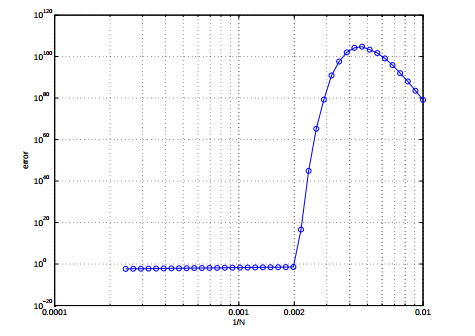
\includegraphics[width=0.8\linewidth]{img/figura_enunciado.png}
\end{center}

¿Cuál es el valor de λ?

\solution

La gráfica nos muestra que se produce un cambio brusco en el error en $h_1=0,2$

Puesto que estamos empleando el método de Euler sabemos que el dominio de estabilidad está formado por todos los puntos en los que $|1-λh|<1$

Si sabemos que esta desigualdad se rompe en $h_1$ podemos ver que λ=10

\end{problem}